%%
%% Template of the department Very Large Business Applications,
%%    CvO University Oldenburg for scientific papers
%%
%% Created by Dipl.-Inform. Daniel Süpke
%%    For questions, comments, suggestions etc. send an email to:
%%    suepke@wi-ol.de or suepke@gmx.de
%%
%% Version: April 16, 2010
%%
%% Note: Has only been tested with pdflatex, not latex (dvi). Still, there is
%% theoretical support also for latex.
%%
\documentclass[enabledeprecatedfontcommands,12pt]{scrartcl}

%% packages
\usepackage[utf8]{inputenc}       % Standard for Linux
%\usepackage[latin1]{inputenc}    % Standard for Windows
\usepackage{ngerman}              % For German language
\usepackage{fancyhdr}
\usepackage{geometry}
\usepackage{ifpdf}
\usepackage{setspace}             % For line spread
\usepackage[printonlyused, withpage, smaller]{acronym}
\usepackage[authoryear, round, sort]{natbib}
\usepackage{csquotes}
\renewcommand{\mkbegdispquote}[2]{\itshape}
\usepackage{enumitem}
\usepackage[table]{xcolor}

% For pdflatex
\ifpdf
  % One of these two:
  \usepackage[pdftex]{graphicx}
  %\usepackage[pdftex]{epsfig}

  \usepackage[pdftex]{hyperref}
% For latex (dvi)
\else
  % One of these two:
  \usepackage[dvips]{graphicx}
  %\usepackage[dvips]{epsfig}

  % make the command \href from hyperref available as a 'print only'
  \newcommand{\href}[2]{#2}
\fi

%% Picture options
\graphicspath{{pictures/}}         % Default path to pictures used
\DeclareGraphicsExtensions{.png}   % More extensions can be added

% Hyper ref coloring
\hypersetup{colorlinks, citecolor=black, linkcolor= black, urlcolor=black}

%% Pagestyle options
\pagestyle{fancy}
%\lhead{}
%\chead{}
%\rhead{}
%\lfoot{Daniel Süpke}
%\cfoot{}
%\rfoot{}
\renewcommand{\headrulewidth}{0.4pt}

\geometry{a4paper,left=3cm,right=3cm}
%\geometry{a4paper,left=3cm,right=2.5cm}   % Please use these settings for a PhD-thesis

%% Document start
\begin{document}

\pagenumbering{Roman}

% Insert titlepage
%% Title page
\begin{titlepage}
  \begin{centering}
  \begin{figure}[h!]
    \centering
    
\includegraphics[width=310pt]{CvO-Oldenburg-Logo}    % Ggf. Copyright beachten - ansonsten nur für Gebrauch an der CvO
  \end{figure}

  \vspace*{-0.8cm}

  \begin{figure}[h!]
    \centering
    
\includegraphics[width=250pt]{VLBA_waagerecht}    % Ggf. Copyright beachten - ansonsten nur für Gebrauch an der CvO/VLBA
  \end{figure}

  \vspace*{0.4cm}
  
  \textsf{\Huge \textbf{Cloud Computing, Internet of Things, Industrie 4.0, Predictive Maintenance, SCADA, SAP HANA\\}}

  \vspace*{0.5cm}
  \noindent Masterarbeit\\

  \end{centering}
  
  \vspace*{1.5cm}
  \begin{tabbing}
  xxxxxxxxxxxxxxxx\= \kill
  
  % Change me
  \small Themensteller:\> Prof. Dr.-Ing. Jorge Marx Gómez\\
  \small Betreuer:\> Prof. Dr.-Ing. Hergen Pargmann\\\\

  \small Vorgelegt von: \>Nils Lutz\\
  \small \>Erlenweg 5\\
  \small \>26129 Oldenburg\\
  \small \>+49 173 25 28 407\\
  \small \>nils.lutz@uni-oldenburg.de\\\\

  \small Abgabetermin:\> 30. April 2017
  \end{tabbing}
\end{titlepage}
%\thispagestyle{empty}
\newpage

% Insert table of contents
% Insert table of contents
\tableofcontents
\newpage

% Insert glossary, table of symbols, list of figures and list of tables
\section*{Akronyme}            % Alternatively a glossary package can be used
\addcontentsline{toc}{section}{Akronyme}
\begin{acronym}[HACCP]
  \acro{api}[API]{Application Programming Interface}
	\acro{baas}[BaaS]{Blockchain-as-a-Service}
  \acro{bft}[BFT]{Byzantine Fault Tolerant}
  \acro{bna}[BNA]{Business Network Archive}
  \acro{brc}[BRC]{British Retail Consortium}
	\acro{btc}[BTC]{Bitcoin}
  \acro{ca}[CA]{Certificate Authority}
  \acro{cli}[CLI]{Command Line Interface}
	\acro{dena}[dena]{Deutsche Energie-Agentur}
	\acro{dlt}[DLT]{Distributed Ledger Technology}
  \acro{dsgvo}[DSGVO]{Datenschutz-Grundverordnung}
  \acro{edi}[EDI]{Electronic Data Interchange}
  \acro{erp}[ERP]{Enterprise Resource Planning}
  \acro{gbt}[GBT]{Global Batch Traceability}
  \acro{gfsi}[GFSI]{Global Food Safety Initiative}
  \acro{gln}[GLN]{Global Location Number}
  \acro{gps}[GPS]{Global Positioning System}
  \acro{haccp}[HACCP]{Hazard Analysis and Critical Control Points}
  \acro{hmsc}[HMSC]{Halal Meat Supply Chain}
  \acro{http}[HTTP]{Hypertext Transfer Protocol}
  \acro{idoc}[IDoc]{Intermediate Document}
  \acro{ifs}[IFS]{International Food Standard}
  \acro{iln}[ILN]{Internationale Lokationsnummer}
	\acro{iot}[IoT]{Internet of Things}
  \acro{ki}[KI]{künstliche Intelligenz}
  \acro{lkv}[LKV]{Los-Kennzeichnungs-Verordnung}
  \acro{lmbg}[LMBG]{Lebensmittel- und Bedarfsgegenständegesetz}
  \acro{lmkv}[LMKV]{Lebensmittelkennzeichnungsverordnung}
	\acro{ml}[ML]{Machine Learning}
  \acro{msp}[MSP]{Member Ship Provider}
  \acro{pbft}[pBFT]{Practical Byzantine Fault Tolerant}
  \acro{pki}[PKI]{Public-Key-Infrastructure}
  \acro{poet}[PoET]{Proof-of-Elapsed-Time}
  \acro{pos}[PoS]{Proof-of-Stake}
  \acro{posp}[PoSp]{Proof-of-Space}
	\acro{pow}[PoW]{Proof-of-Work}
  \acro{reif}[REIF]{Resource-Efficent, Economic and Intelligent Foodchain}
  \acro{rest}[REST]{Representational State Transfer}
  \acro{rfid}[RFID]{Radiofrequenz-Identifikation}
	\acro{sc}[SC]{Smart Contract}
  \acro{sql}[SQL]{Structured Query Language}
  \acro{tls}[TLS]{Transport Layer Security}
  \acro{tms}[TMS]{Transportation Management System}
  \acro{ui}[UI]{User Interface}
  \acro{uri}[URI]{Uniform Resource Identifier}
  \acro{vvvo}[VVVO]{Vieh-Verkehrs-Verordnung}
  \acro{wms}[WMS]{Wharehouse Management System}
  \acro{xml}[XML]{Extensible Markup Language}
\end{acronym}

% \section*{Symbolverzeichnis}   % If needed
% \addcontentsline{toc}{section}{Symbolverzeichnis}
\newpage

\listoffigures
\addcontentsline{toc}{section}{Abbildungsverzeichnis}
\listoftables
\addcontentsline{toc}{section}{Tabellenverzeichnis}
\lstlistoflistings
\addcontentsline{toc}{section}{Quelltextverzeichnis}
\newpage


\pagenumbering{arabic}

%% Line spread
\onehalfspacing

% Insert introduction
\section{Motivation}

Industrie 4.0 ist ein Treiber der Digitalisierung vor allem im Bereich der Energiewirtschaft. \cite[vgl.]{UnternehmensbetreuungmbH2017} Durch den Einsatz von Industrie 4.0 sind Unternehmen in der Lage ihre Prozesse und Anlagen in Echtzeit Kontrollieren und Steuern zu können. Dadurch lassen sich Kosten optimieren und die Produktivität steigern. Industrie 4.0 ist der Oberbegriff für eine viel zahl von Technologien.\\
Eine Technologie die bereits heute neue innovative Ideen im privaten Sektor hervorgebracht hat, erobert den industriellen Sektor - Blockchain. Eine Blockchain ist eine verteilte Datenstruktur kombiniert mit Kryptographischen Methoden zur Sicherstellung der Unveränderbarkeit der Daten. Blockchains zählen zu den \ac{dlt}. So erwägen einige der größten Finanzinstitutionen den Einsatz von \ac{dlt}.\cite{Goldman2018}\cite{JPMorgan2018}\\

“Es ist davon auszugehen, dass wir in ein bis zwei Jahrzehnten wirtschaftlich über Mechanismen miteinander interagieren werden, für die wir bislang weder Konzepte noch Begriffe haben.” \cite[S.~92]{Platzer2014} Auch die Deutsche Bundesregierung ist an der Blockchain Technologie interessiert und erwägt den Einsatz in der Zukunft für die unterschiedlichsten Services. In einer der jüngsten Pressemitteilungen hat der Blockchain Bundesverband mitgeteilt, dass die Regierung eine umfassende Strategie zum Umgang und Einsatz der Technologie erarbeiten will. \cite{BCBundesverband2018}

\begin{figure}[h!]
	\centering
	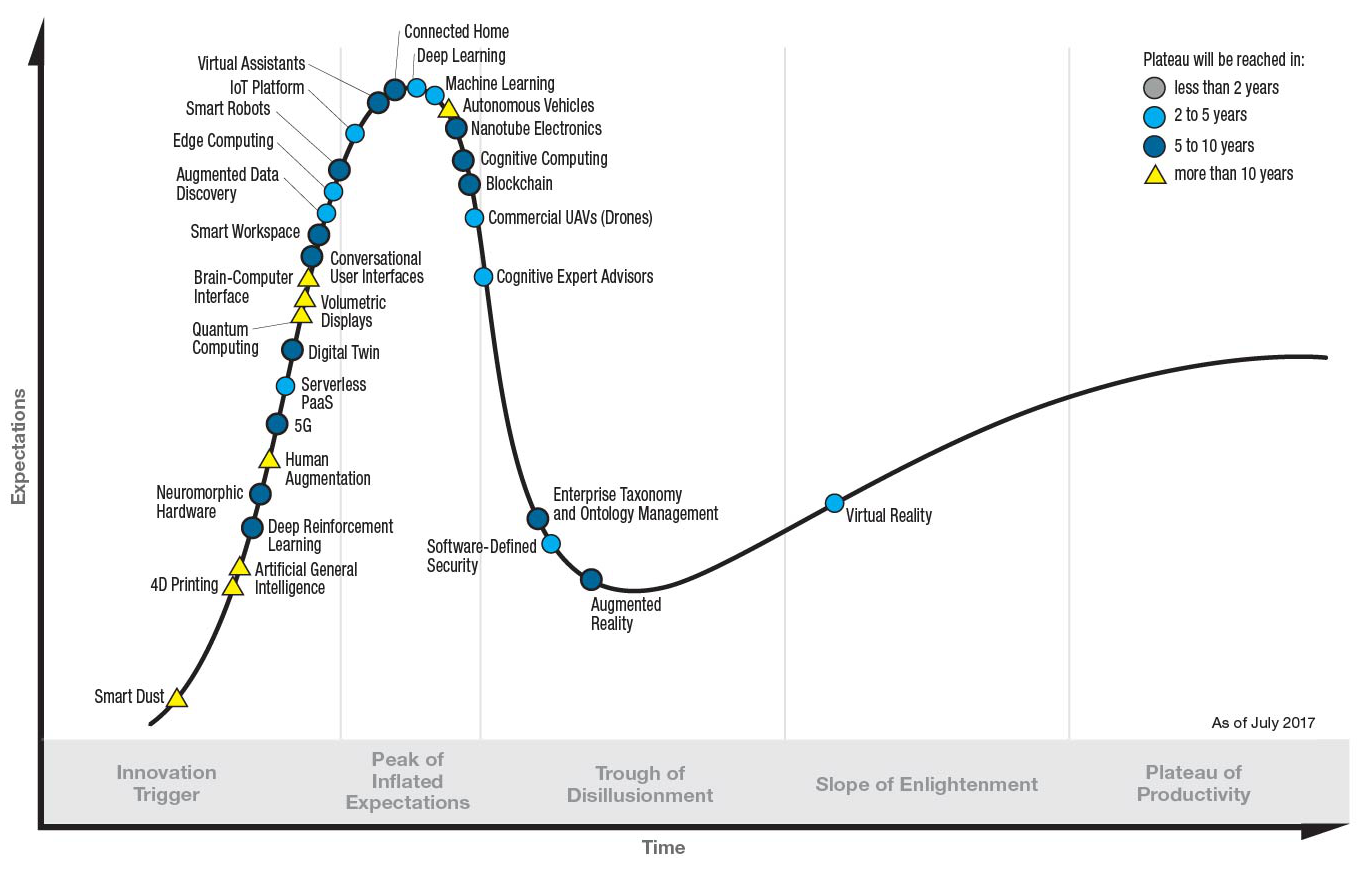
\includegraphics[width=0.65\linewidth]{pictures/Gartner-Hype-Cycle-2017}
	\caption[Gartner Hype Cycle 2017]{Emerging Technologies Hype Cycle 2017\cite{Gartner2017}}
	\label{fig:gartner-hype-cycle-2017}
\end{figure}

Noch ist die Blockchain kein Alltag, bemessen am jährlich erscheinenden Hype Cycle des Marktforschungsinstituts Gartner, Inc. $( Abb.~ \ref{fig:gartner-hype-cycle-2017} )$ hat die Technologie noch fünf bis zehn Jahre Entwicklungszeit vor sich. Erst dann wird sie nach aktueller Einschätzung im produktiven Einsatz sein. Was der Hype Cycle nicht aussagt ist welchen Einfluss die Blockchain auf eine Branche oder die Gesellschaft hat in ihrer jeweiligen Phase.\\

Bereits heute zeigen sich signifikante Unterschiede zwischen den unzähligen Blockchains die in Pilotprojekten realisiert wurden. So gibt es Anwendungen der Blockchain um beispielsweise den Kilometerstand eines Fahrzeugs täglich \glqq in die Blockchain\grqq~ zu schreiben. Die inhärenten Eigenschaften der Blockchain ermöglichen es sehr einfach festzustellen, ob ein Kilometerstand nachträglich durch Fremdeinwirkung manipuliert wurde. Ebenfalls ist keine zentrale Zwischenstelle mehr nötig, um für die Echtheit des hinterlegten Wertes zu garantieren. \cite{carVertical}\\

Bitcoin war die erste Generation von Blockchain. Die Bitcoin Blockchain ist in der Lage Einheiten der Bitcoin Währung zwischen zwei Parteien zu versenden ohne das eine Bank oder eine Clearingstelle diese Transaktion validieren muss. \cite[vgl.]{Nakamoto2009} Ethereum war die zweite Generation einer Blockchain. Im Vergleich zur Bitcoin Blockchain lassen sich mit dem Ethereum Netzwerk auch sog. \ac{sc} erstellen und ausführen.\cite[vgl.]{Buterin2014} Mittlerweile behaupten die ersten Projekte von sich zur dritten Generation von Blockchains zu gehören. Skalierbarkeit und Interoperabilität spielen in dieser Generation eine der entscheidenden Rollen. \cite[vgl.]{Cardano} Auch die Blockchain Anwendungen im Enterprise Bereich lassen in Masse noch auf sich warten. Es fehlen Erfahrungen und konkrete Einsatzgebiete für die Technologie.

\newpage


% Insert body
\section{Problemstellung}

Soll die Blockchain Technologie zum Einsatz kommen gibt es offene Fragen. Eine Blockchain ist keine Silberkugel für sämtliche betriebswirtschaftliche Prozesse. Viel mehr kann eine Blockchain als Skalpell dienen um präzise ein bestimmtes Problem zu lösen.\\
Der technische Hintergrund einer Blockchain ist nicht neu. Die einzelnen Komponenten sind bereits heute vielfach erprobt im produktiven Einsatz.\cite{Diffie1976}\cite{Steinmetz2005} Die Kombination zu einer Blockchain ist allerdings neu und aktuell nur in Pilotprojekten für vereinzelte Use-cases zu finden.

\begin{figure}[h!]
	\centering
	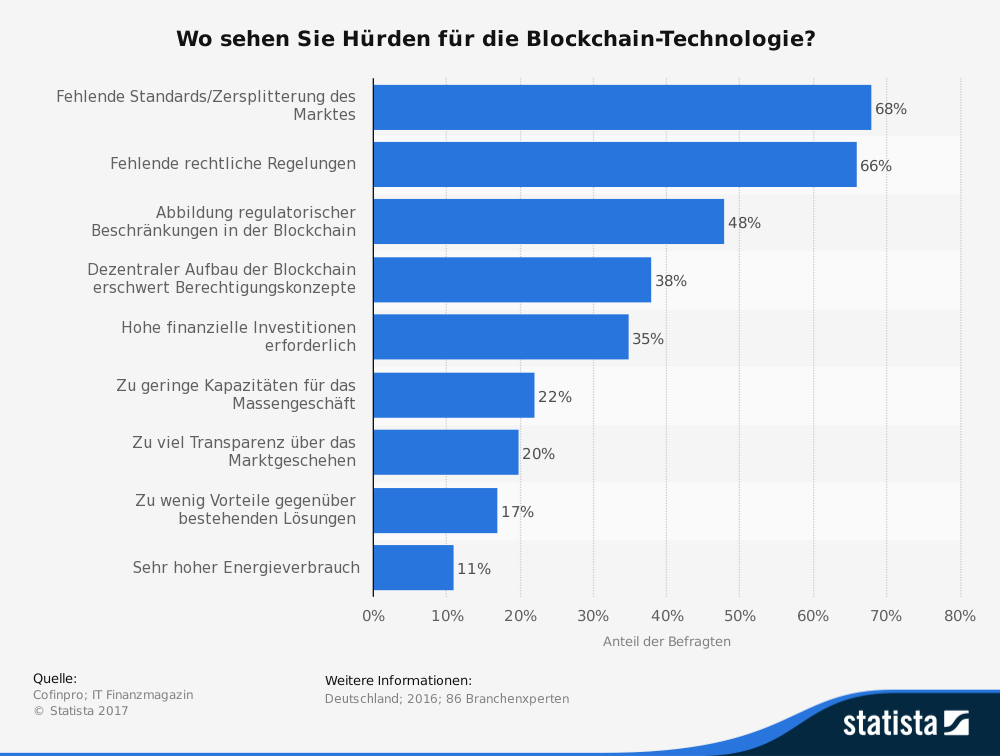
\includegraphics[width=0.9\linewidth]{pictures/Statista-Huerden-Blockchain-2016}
	\caption[Statista Blockchain Umfrage]{Cofinpro - Wo sehen Sie Hürden für die Blockchain Technologie?\cite{Cofinpro}}
	\label{fig:statista-huerden-blockchain-2016}
\end{figure}

Abbildung \ref{fig:statista-huerden-blockchain-2016} zeigt die Ergebnisse einer Umfrage des Fachmagazins Cofinpro zum Thema \glqq Wo sehen Sie Hürden für die Blockchain-Technologie?\grqq~. So scheinen die mit Abstand größten Einstiegsbarrieren fehlende Standards und rechtliche Regelungen zu sein.

%Die Kernidee hinter der Blockchain-Technologie ist es einen Intermediär zu substituieren, der nur eingesetzt wurde um eine neutrale Vertrauensbildung zu ermöglichen. \ac{dlt} verfolgt dabei den Ansatz die Vertrauensbildung, den Ablauf von Transaktionen und deren sichere Festschreibung mit mathematischen und kryptographischen Methoden zu realisieren. Im Kontrast zum konventionellen Intermediär, welcher durch eine dritte Person oder Institution wie z.B. eine Bank oder einen Notar repräsentiert wird.\\
%
%Für das Problem der Einigkeit über den Zustand eines Werts innerhalb der Blockchain sind zwei generelle Verfahren etabliert. Die \ac{pow} und \ac{pos} genannten Algorithmen nutzen unterschiedliche Ansätze um Konsens innerhalb eines Netzwerks zu bilden und so Vertrauen herzustellen. Beide Verfahren haben ihre Vor- und Nachteile.

Betrachtet man die Energiewirtschaft findet man genügend Prozesse die einen transaktionalen Charakter besitzen und oft auch ein oder mehrere Vermittlerstellen zwischengeschaltet haben. Fehlende Standards und generelle Unsicherheit verhindern allerdings den flächendeckenden Einsatz einer Blockchain. Obwohl die Technologie im Bereich der Plattformen und Prozesse in einigen Anwendungsfeldern mindestens unterstützend vermutlich aber sogar ersetzend eingesetzt werden kann.\\

Die \ac{dena} hat zusammen mit der privaten Hochschule ESMT Berlin von Führungskräften der deutschen Energiewirtschaft einschätzen lassen welche Bereiche und wie groß die Potentiale durch Blockchain-Technologie jeweils sind. Abbildung \ref{fig:dena-blockchain-use-cases} zeigt schematisch das Ergebnis, wobei eine dunklere Färbung eine höhere Übereinstimmung zwischen Herausforderung und Lösungsansatz mit Blockchain und die Größe der Kreise die Wahrscheinlichkeit für einen Einsatz in naher Zukunft zeigen. Der Umfrage ist zu entnehmen, dass über die Hälfte der Teilnehmer eine weitere Verbreitung von Blockchain Technologie in der Energiewirtschaft für wahrscheinlich halten.\cite[vgl.]{EnergieAgentur2016}

\begin{figure}[h!]
	\centering
	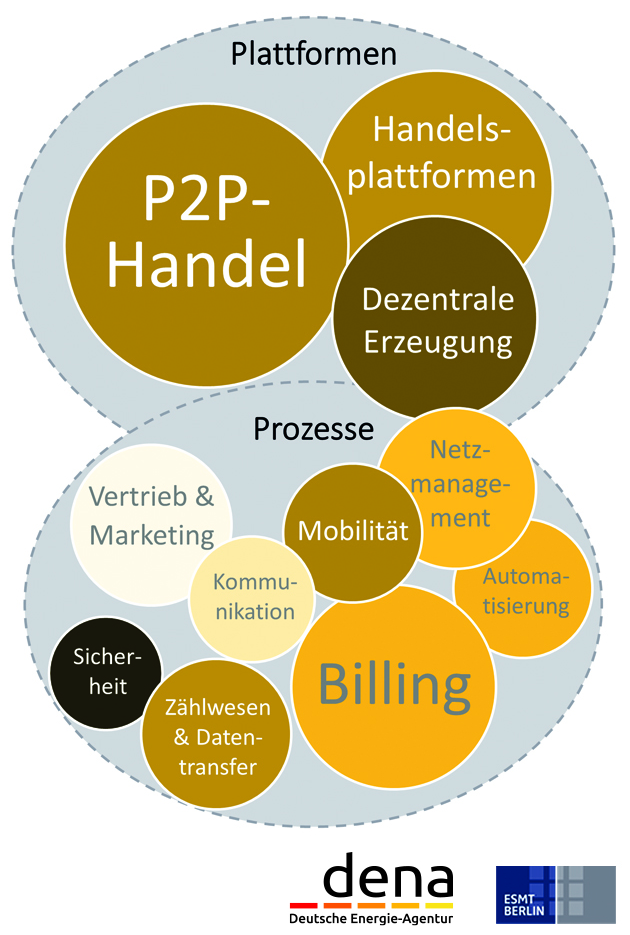
\includegraphics[width=0.41\linewidth]{pictures/dena-blockchain-use-cases}
	\caption[dena Potentielle Anwendungsfelder der Blockchain]{Potentielle Anwendungsfelder der Blockchain\cite{EnergieAgentur2016}}
	\label{fig:dena-blockchain-use-cases}
\end{figure}

%\begin{itemize}
%	\item Technologie ist so neu und frisch verfügbar im Industriekontext
%	\item Ermittlung und Definition möglicher Geschäftsprozesse der Energiewirtschaft
%	\item Vorhandene Lösungen am Markt vergleichen für den Einsatz
%	\item Mehrwert eines DLT-basierten Geschäftsprozesses herausarbeiten
%	\item Spieltheorie neue Geschäftsfelder Blockchain
%\end{itemize}

%Video [Wir und die Blockchain (The Blockchain and Us) (2017) - Deutsche Synchronfassung/German version - YouTube](\url{https://www.youtube.com/watch?v=x2mKDWsNijo})

% konkrete Beschreibung des Problems

\newpage
\section{Vorgehen / Methodik}

Die beschriebenen Probleme und Ziele sollen gelöst und erreicht werden mittels der sog. Design Science Methode nach Hevner \citep{Hevner2004}.

\newpage

\section{Ziele}

Der Einsatz von \textit{Blockchain-Technologie} könnte - für die in Kapitel \ref{Problemstellung} beschriebene Problemstellung - eine Lösung darstellen. Eine \textit{Blockchain} ist ein dezentrales System zur manipulationssicheren Speicherung von Informationen in sog. \textit{Blöcken} die untereinander durch kryptographische Methoden verkettet sind - daher auch der Name \textit{Blockchain}. Eine \textit{Blockchain} verwendet verschiedenste Verfahren zur Konsensbildung innerhalb des Netzwerks, um sicherzustellen das neue \textit{Blöcke} und die darin enthaltenen Transaktionen vom gesamten Netzwerk validiert und verifizert werden bevor der \textit{Block} in die \textit{Blockchain} geschrieben wird \citep[siehe auch][]{Nakamoto2009, Buterin2014, Cardano2017, carVertical}.

Außerdem kann eine \textit{Blockchain} durch den Einsatz einer kryptographischen \textit{Hashfunktion}\footnote{Spezielle Form einer Hashfunktion, welche kollisionsresistent ist. Es ist praktisch nicht möglich, zwei unterschiedliche Eingabewerte zu finden, die einen identischen Hashwert ergeben \citep{Menezes1997}.} zur Bildung einer Prüfsumme für jeden \textit{Block} innerhalb der \textit{Blockchain} sicherstellen, dass bereits persistierte Informationen nicht ohne weiteres manipuliert werden können. Im Idealfall ist eine \textit{Blockchain} dezentral konzipiert, was bedeutet, das jeder Teilnehmer eines \textit{Blockchain} Netzwerks eine exakte Kopie des Datenbestands lokal vorhält. Hierdurch soll sichergestellt werden, das auch bei einem Ausfall oder einer Kompromittierung einzelner Teilnehmer das Gesamtsystem weiterhin in seiner Funktion stabil bleibt \citep{Drescher2017, Tribis2018}.\\

Ziel dieser Arbeit ist es, durch Entwicklung und Evaluation eines Prototyps die Möglichkeiten und Grenzen der \textit{Blockchain-Technologie} im Kontext der Chargenrückverfolgung in der Fleischwarenindustrie zu überprüfen. Dabei sollen die dafür nötigen Daten und Informationen ermittelt und in einen Systementwurf eingearbeitet werden. Außerdem ist angestrebt aus der vielzahl von unterschiedlichen Implementierungen einer \textit{Blockchain} genau die Ausprägung zu identifizieren, welche für die spezifischen Anforderungen der Fleischwarenindustrie ideal erscheint.

Konkret lassen sich hieraus folgende Ziele und erwartete Ergebnisstypen zu den jeweiligen Forschungsfragen aus Kapitel \ref{Problemstellung} ableiten.

\begin{itemize}
  \item Identifikation verwandter Arbeiten aus Wissenschaft und Praxis für FF1.1
  \item Anforderungserhebung und -analyse mit dem Praxispartner für FF1.1
  \begin{itemize}
    \item Funktional
    \item Qualitativ
    \item Rahmenbedingungen
  \end{itemize}
  \item Prozessaufnahme und -analyse für FF1.2
  \begin{itemize}
    \item Schwachstellenanalyse des \textit{Ist}-Prozess
    \item Modellierung eines \textit{Soll}-Prozess bei Einsatz von \textit{Blockchain-Technologie}
  \end{itemize}
  \item SWOT-Analyse als Vorbereitung für eine Nutzwertanalyse zur Klärung von FF1.3
  \item Ableitung eines Systementwurfs mittels Design Science Research für FF1.4
  \item Entwicklung eines Prototyps anhand der Ergebnisse von FF1.1-4 für FF1
  \item Evaluation des Prototyps durch Experteninterview für FF1
\end{itemize}

Der enstandene Prototyp soll beim Praxispartner Westfleisch SCE mbH als Entscheidungshilfe für eine zukünftige Innovationsstrategie zur Optimierung der Lieferkette dienen.

% Ziel dieser Arbeit ist es, die theoretischen Grundlagen der \textit{Blockchain-Technologie} darzulegen und nachzuweisen, ob sie auf die Fleischwarenindustrie übertragbar sind, um den Aufbau eines Systems zur Chargenrückverfolgung zu evaluieren. Dafür sollen die spezifischen Anforderungen der Branche durch Experteninterviews ermittelt werden und eine erste Schnittstellenbeschreibung entstehen die es ermöglicht neuen Teilnehmern der Lieferkette unkompliziert am Netzwerk teilzunehmen. Auf dieser Basis soll dann in einer prototypischen Umsetzung die Machbarkeit der Anwendung von \textit{Blockchain-Technologie} in der Nahrungsmittelindustrie überprüft bzw. evaluiert werden.\\

% Im Vordergrund des Prototyps stehen Aspekte wie Prozesssicherheit, Schutz vor Manipulation durch Teilnehmer und Externe wie auch Möglichkeiten der Geheimhaltung von Geschäftsgeheimnissen bei maximaler Transparenz für alle Teilnehmer.\\

% Der technische Hintergrund einer \textit{Blockchain} ist nicht neu. Die einzelnen Komponenten sind bereits heute vielfach erprobt im produktiven Einsatz. \citep{Diffie1976}\citep{Steinmetz2005} Die Kombination zu einer \textit{Blockchain} ist allerdings neu und aktuell nur in Pilotprojekten für vereinzelte Use-cases zu finden.\\

\newpage

\section{Vorläufige Gliederung}
\begin{small}
	1. Einleitung\\
	\noindent\hspace*{10mm}%
	1.1. Motivation\\
	\noindent\hspace*{10mm}%
	1.2. Problemstellung\\
	\noindent\hspace*{10mm}%
	1.3. Lösungsansatz\\
	\noindent\hspace*{10mm}%
	1.4. Struktur der Arbeit\\
	2. Grundlagen Chargenrückverfolgung in der Nahrungsmittelindustrie\\
	\noindent\hspace*{10mm}%
	3.1. ABC\\
	\noindent\hspace*{10mm}%
	3.2. XYZ\\
	\noindent\hspace*{10mm}%
	3.3. ÄÖÜ\\
	3. Grundlagen Blockchain\\
	\noindent\hspace*{10mm}%
	3.1. Definition\\
	%2.1.1. Blockchain\\
	%2.1.2. Tangle\\
	%2.1.3. Hash Graph\\
	%2.1.4. Distributed Ledger\\
	\noindent\hspace*{10mm}%
	3.2. Arten von DLT\\
	%2.2.1. Public\\
	%2.2.2. Private\\
	%2.2.3. Consortium\\
	\noindent\hspace*{10mm}%
	3.3. Abgrenzung zu Cryptocurrencies\\
	\noindent\hspace*{10mm}%
	3.4. Technologischer Aufbau\\
	%2.4.1. Sicherheit\\
	%2.4.1.1. Public-Key Authorization\\
	%2.4.1.2. Hashing Algorithm\\
	%2.4.2. Consensus Algorithm\\ https://www.btc-echo.de/konsens-vs-regierung-warum-bitcoin-keine-demokratie-ist/
	%2.4.3. Dezentralisierung\\
	%2.4.3.1. Peer-to-Peer Netzwerke\\
	%2.4.3.2. Shared Computing\\
	\noindent\hspace*{10mm}%
	3.5. Ausprägungen von DLTs\\
	%2.5.1. Bitcoin Blockchain\\
	%2.5.2. Ethereum Blockchain\\
	%2.5.2.1. Ethereum\\
	%2.5.2.2. Ethereum Enterprise Alliance\\
	%2.5.3. Iota Tangle\\
	%2.5.4. Ripple\\
	%2.5.5. IBM Bluemix\\
	%2.5.6. Microsoft Azure\\
	%2.5.7. SAP Leonardo\\
	%2.5.8. Hyperledger\\
	4. Blockchain Technologie in der Nahrungsmittelindustrie\\
	\noindent\hspace*{10mm}%
	4.1. Funktionale Anforderunggen\\
	%4.1.1. SWOT-Analyse\\
	%4.1.2. Entscheidungsbaum\\
	\noindent\hspace*{10mm}%
	4.2. Nicht-Funktionale Anforderunggen\\
	%4.2.1. Transaktional\\
	%4.2.2. Geschwindigkeit\\
	%4.2.3. Transparenz\\
	%4.2.4. Vertrauen\\
	%4.2.5. Unveränderlichkeit\\
	%4.2.6. Geschäftsregeln\\
	\noindent\hspace*{10mm}%
	4.3. Mehrwerte durch DLT\\
	%4.3.1. Transaktionskosten senken\\
	%4.3.2. Transaktionsgeschwindigkeit erhöhen\\
	%4.3.3. Datenverfügbarkeit über die gesamte Supply Chain erhöhen\\
	%4.3.4. Neue innovative Geschäftsmodelle ermöglichen\\
	5. Prototypische Umsetzung\\
	\noindent\hspace*{10mm}%
	5.1 Environment\\
	%5.2.1. Business Network\\
	%5.2.2. Security\\
	%5.2.3. Cloud Resources\\
	\noindent\hspace*{10mm}%
	5.2 Development\\
	%5.3.1. Tools\\
	%5.3.2. Listings\\
	\noindent\hspace*{10mm}%
	5.3 Deployment\\
	6. Fazit\\
\end{small}

\newpage



% Insert conclusion
\section{Zeitplanung}
Zwei flinke Boxer jagen die quirlige Eva und ihren Mops durch Sylt. Franz jagt im komplett verwahrlosten Taxi quer durch Bayern. Zwölf Boxkämpfer jagen Viktor quer über den großen Sylter Zwei flinke Boxer jagen die quirlige Eva und ihren Mops durch Sylt. Franz jagt im komplett verwahrlosten Taxi quer durch Bayern. Zwölf Boxkämpfer jagen Viktor quer über den großen Sylter Deich. Vogel Quax zwickt Johnys Pferd Bim. Sylvia wagt quick den Jux bei Pforzheim. Polyfon zwitschernd aßen Mäxchens Vögel Rüben, Joghurt und Quark.\\
"`Fix, Schwyz!"' quäkt Jürgen blöd vom Paß. Victor jagt zwölf Boxkämpfer quer über den großen Sylter Deich. Falsches Üben von Xylophonmusik quält jeden größeren Zwerg. Heizölrückstoßabdämpfung. Zwei flinke Boxer jagen die quirlige Eva und ihren Mops durch Sylt. Franz jagt im komplett verwahrlosten Taxi quer durch Bayern.\\
Zwölf Boxkämpfer jagen Viktor quer über den großen Sylter Deich. Vogel Quax zwickt Johnys Pferd Bim. Sylvia wagt quick den Jux bei Pforzheim. Polyfon zwitschernd aßen Mäxchens Vögel Rüben, Joghurt und Quark. "`Fix, Schwyz!"' quäkt Jürgen blöd vom Paß. Victor jagt zwölf Boxkämpfer quer über den großen Sylter Deich.\\


\newpage

\pagenumbering{Roman}
\setcounter{page}{3}

% Insert appendix
\begin{appendix}

\addcontentsline{toc}{section}{Literaturverzeichnis}
\bibliographystyle{alpha}
\bibliography{thesis} % Point to BibTeX literature file e.g. literatur.bib

\end{appendix}
\newpage


\end{document}
